% Chapter 3: Seminar - ARIMA Models
% Harvard-quality academic presentation
% Bachelor program, Bucharest University of Economic Studies

\documentclass[9pt, aspectratio=169, t]{beamer}

% Ensure content fits on slides
\setbeamersize{text margin left=8mm, text margin right=8mm}

%=============================================================================
% THEME AND STYLE CONFIGURATION
%=============================================================================
\usetheme{default}
% Using default theme for clean header/footer control

% Color Palette (matching Redispatch PDF)
\definecolor{MainBlue}{RGB}{26, 58, 110}
\definecolor{AccentBlue}{RGB}{26, 58, 110}
\definecolor{IDAred}{RGB}{205, 0, 0}
\definecolor{DarkGray}{RGB}{51, 51, 51}
\definecolor{MediumGray}{RGB}{128, 128, 128}
\definecolor{LightGray}{RGB}{248, 248, 248}
\definecolor{VeryLightGray}{RGB}{235, 235, 235}
\definecolor{KeynoteGray}{RGB}{218, 218, 218}
\definecolor{SectionGray}{RGB}{120, 120, 120}
\definecolor{FooterGray}{RGB}{100, 100, 100}
\definecolor{Crimson}{RGB}{220, 53, 69}
\definecolor{Forest}{RGB}{46, 125, 50}
\definecolor{Amber}{RGB}{181, 133, 63}
\definecolor{Orange}{RGB}{230, 126, 34}
\definecolor{Purple}{RGB}{142, 68, 173}

% Gradient background (exact Keynote 315° gradient: white to RGB 218,218,218)
\setbeamertemplate{background}{%
    \begin{tikzpicture}[remember picture, overlay]
        \shade[shading=axis, shading angle=315,
        top color=white, bottom color=KeynoteGray]
        (current page.south west) rectangle (current page.north east);
    \end{tikzpicture}%
}
% Fallback solid color for compatibility
\setbeamercolor{background canvas}{bg=}

\setbeamercolor{palette primary}{bg=MainBlue, fg=white}
\setbeamercolor{palette secondary}{bg=MainBlue!85, fg=white}
\setbeamercolor{palette tertiary}{bg=MainBlue!70, fg=white}
\setbeamercolor{structure}{fg=MainBlue}
\setbeamercolor{title}{fg=IDAred}
\setbeamercolor{frametitle}{fg=IDAred, bg=}
\setbeamercolor{block title}{bg=MainBlue, fg=white}
\setbeamercolor{block body}{bg=VeryLightGray, fg=DarkGray}
\setbeamercolor{block title alerted}{bg=Crimson, fg=white}
\setbeamercolor{block body alerted}{bg=Crimson!8, fg=DarkGray}
\setbeamercolor{block title example}{bg=Forest, fg=white}
\setbeamercolor{block body example}{bg=Forest!8, fg=DarkGray}
\setbeamercolor{item}{fg=MainBlue}

% Footer colors (override Madrid theme blue)
\setbeamercolor{author in head/foot}{fg=FooterGray, bg=}
\setbeamercolor{title in head/foot}{fg=FooterGray, bg=}
\setbeamercolor{date in head/foot}{fg=FooterGray, bg=}
\setbeamercolor{section in head/foot}{fg=FooterGray, bg=}
\setbeamercolor{subsection in head/foot}{fg=FooterGray, bg=}

% Bullet styles (apply everywhere including blocks)
\setbeamertemplate{itemize item}{\color{MainBlue}$\boxdot$}
\setbeamertemplate{itemize subitem}{\color{MainBlue}$\blacktriangleright$}
\setbeamertemplate{itemize subsubitem}{\color{MainBlue}\tiny$\bullet$}
\setbeamertemplate{itemize/enumerate body begin}{\normalsize}
\setbeamertemplate{itemize/enumerate subbody begin}{\normalsize}

% Item spacing - compact style
\setlength{\leftmargini}{10pt}       % Level 1: minimal indent
\setlength{\leftmarginii}{10pt}      % Level 2: minimal additional indent
% Compact list spacing (zero extra space before/after lists in blocks)
\makeatletter
\def\@listi{\leftmargin\leftmargini \topsep 0pt \parsep 0pt \itemsep 0pt}
\def\@listii{\leftmargin\leftmarginii \topsep 0pt \parsep 0pt \itemsep 0pt}
\makeatother

\setbeamertemplate{navigation symbols}{}

%=============================================================================
% CUSTOM HEADLINE
%=============================================================================
\setbeamertemplate{headline}{%
    \vskip10pt%
    \hbox to \paperwidth{%
        \hskip0.5cm%
        {\small\color{FooterGray}\renewcommand{\hyperlink}[2]{##2}\insertsectionhead}%
        \hfill%
        \textcolor{FooterGray}{\small\insertframenumber}%
        \hskip0.5cm%
    }%
    \vskip4pt%
    {\color{FooterGray}\hrule height 0.4pt}%
}

%=============================================================================
% CUSTOM FOOTER
%=============================================================================
\usepackage{fontawesome5}

\setbeamertemplate{footline}{%
    {\color{FooterGray}\hrule height 0.4pt}%
    \vskip4pt%
    \hbox to \paperwidth{%
        \hskip0.5cm%
        \textcolor{FooterGray}{\small Time Series Analysis and Forecasting}%
        \hfill%
        \raisebox{-0.1em}{%
            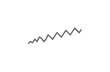
\begin{tikzpicture}[x=0.08em, y=0.08em, line width=0.4pt]
                \draw[FooterGray] (0,3) -- (1,4) -- (2,3.5) -- (3,5) -- (4,4) -- (5,6) -- (6,5.5) -- (7,4) -- (8,5) -- (9,7) -- (10,6) -- (11,5) -- (12,6.5) -- (13,8) -- (14,7) -- (15,6) -- (16,7.5) -- (17,9) -- (18,8) -- (19,7) -- (20,8.5) -- (21,10) -- (22,9) -- (23,8) -- (24,9.5);
            \end{tikzpicture}%
        }%
        \hskip0.5cm%
    }%
    \vskip6pt%
}

%=============================================================================
% PACKAGES
%=============================================================================
\usepackage[utf8]{inputenc}
\usepackage[T1]{fontenc}
\usepackage[english]{babel}
\usepackage{amsmath, amssymb, amsthm}
\usepackage{mathtools}
\usepackage{bm}
\usepackage{tikz}
\usetikzlibrary{arrows.meta, positioning, shapes, calc, decorations.pathreplacing, shadings}
\usepackage{booktabs}
\usepackage{multirow}
\usepackage{array}
\usepackage{graphicx}
\usepackage{hyperref}
\usepackage{colortbl}
\hypersetup{colorlinks=true, linkcolor=MainBlue, urlcolor=MainBlue}
\graphicspath{{../../logos/}{../../charts/}}
\hfuzz=2pt  % Suppress tiny overfull warnings (<2pt)
\vfuzz=2pt  % Suppress tiny vertical overfull warnings (<2pt)

%=============================================================================
% QUANTLET COMMAND
%=============================================================================
\newcommand{\quantlet}[2]{%
    \hfill\href{#2}{%
        \raisebox{-0.15em}{\includegraphics[height=0.7em]{ql_logo.png}}%
        \textcolor{MainBlue}{\tiny\ #1}%
    }%
}

%=============================================================================
% THEOREM ENVIRONMENTS
%=============================================================================
\theoremstyle{definition}
\setbeamertemplate{theorems}[numbered]
\newtheorem{defn}{Definition}
\newtheorem{thm}{Theorem}
\newtheorem{prop}{Proposition}
\newtheorem{rmk}{Remark}

%=============================================================================
% CENTRED MINIPAGE (no extra vertical space)
%=============================================================================
\newenvironment{cminipage}[1]{%
    \par\noindent\hfill\begin{minipage}{#1}\ignorespaces
}{%
    \end{minipage}\hfill\null\par
}

%=============================================================================
% CUSTOM COMMANDS
%=============================================================================
\newcommand{\E}{\mathbb{E}}
\newcommand{\Var}{\text{Var}}
\newcommand{\Cov}{\text{Cov}}
\newcommand{\Corr}{\text{Corr}}
\newcommand{\R}{\mathbb{R}}
\newcommand{\N}{\mathbb{N}}
\newcommand{\Z}{\mathbb{Z}}
\newcommand{\RMSE}{\text{RMSE}}
\newcommand{\MAE}{\text{MAE}}
\newcommand{\MAPE}{\text{MAPE}}

% Quiz styling
\newcommand{\correct}{\textcolor{Forest}{\checkmark}}
\newcommand{\incorrect}{\textcolor{Crimson}{\texttimes}}

%=============================================================================
% CUSTOM TITLE PAGE
%=============================================================================
\defbeamertemplate*{title page}{hybrid}[1][]
{
    \vspace{0.2cm}
    % Logos row - top header (with clickable links)
    \begin{center}
        \href{https://www.ase.ro}{\includegraphics[height=1.0cm]{ase_logo.png}}\hspace{0.3cm}%
        \href{https://theida.net}{\includegraphics[height=1.0cm]{ida_logo.png}}\hspace{0.3cm}%
        \href{https://blockchain-research-center.com}{\includegraphics[height=1.0cm]{brc_logo.png}}\hspace{0.3cm}%
        \href{https://www.ai4efin.ase.ro}{\includegraphics[height=1.0cm]{ai4efin_logo.png}}\hspace{0.3cm}%
        \href{https://ipe.ro/new}{\includegraphics[height=1.0cm]{acad_logo.png}}\hspace{0.3cm}%
        \href{https://www.digital-finance-msca.com}{\includegraphics[height=1.0cm]{msca_logo.png}}%
    \end{center}

    \vspace{0.6cm}

    % Main title with Q logos on sides (with clickable links)
    \begin{center}
        \begin{minipage}{0.1\textwidth}
            \centering
            \href{https://quantlet.com}{\includegraphics[height=1.1cm]{ql_logo.png}}
        \end{minipage}%
        \begin{minipage}{0.78\textwidth}
            \centering
            {\LARGE\bfseries\usebeamercolor[fg]{title}\inserttitle}

            \vspace{0.3cm}

            {\usebeamerfont{subtitle}\usebeamercolor[fg]{title}\insertsubtitle}
        \end{minipage}%
        \begin{minipage}{0.1\textwidth}
            \centering
            \href{https://quantinar.com}{\includegraphics[height=1.1cm]{qr_logo.png}}
        \end{minipage}
    \end{center}

    \vspace{0.6cm}

    % Authors (left aligned)
    \hspace{0.5cm}{\usebeamerfont{author}\insertauthor}

    \vspace{0.3cm}

    % Institute/Affiliations (left aligned)
    \hspace{0.5cm}\begin{minipage}[t]{0.9\textwidth}
        \raggedright\small\insertinstitute
    \end{minipage}
}

%=============================================================================
% TITLE INFORMATION
%=============================================================================
\title[Time Series Analysis]{Time Series Analysis and Forecasting}
\subtitle{Seminar 3: ARIMA Models}
\author[D.T. Pele]{Daniel Traian PELE}
\institute{Bucharest University of Economic Studies\\
IDA Institute Digital Assets\\
Blockchain Research Center\\
AI4EFin -- Artificial Intelligence for Energy Finance\\
Romanian Academy, Institute for Economic Forecasting\\
MSCA Digital Finance}
\date{}

\begin{document}

% Title page (no header/footer)
{
\setbeamertemplate{headline}{}
\setbeamertemplate{footline}{}
\begin{frame}
    \titlepage
\end{frame}
}

%=============================================================================
% SEMINAR OUTLINE
%=============================================================================
\section{Overview}

\begin{frame}{Seminar Outline}
    \begin{cminipage}{0.95\textwidth}
    \textbf{\large Today's Activities:}

    \vspace{0.4cm}

    \begin{enumerate}
        \item[\textcolor{MainBlue}{\textbf{1.}}] \textbf{Review Quiz} --- Checking understanding of ARIMA concepts
        \vspace{0.15cm}
        \item[\textcolor{MainBlue}{\textbf{2.}}] \textbf{True/False Questions} --- Conceptual checks
        \vspace{0.15cm}
        \item[\textcolor{MainBlue}{\textbf{3.}}] \textbf{Practice Problems} --- Calculations with ARIMA
        \vspace{0.15cm}
        \item[\textcolor{MainBlue}{\textbf{4.}}] \textbf{Worked Examples} --- Real-world applications
        \vspace{0.15cm}
        \item[\textcolor{MainBlue}{\textbf{5.}}] \textbf{Real Data Analysis} --- GDP case study
        \vspace{0.15cm}
        \item[\textcolor{MainBlue}{\textbf{6.}}] \textbf{AI Exercises} --- Human vs.\ AI modeling
    \end{enumerate}
    \end{cminipage}
\end{frame}

%=============================================================================
% SECTION 1: REVIEW QUIZ
%=============================================================================
\section{Review Quiz}

\begin{frame}{Quiz 1: Integration Order}
    \begin{cminipage}{0.95\textwidth}
    \begin{alertblock}{Question}
        A time series $Y_t$ requires two differences to become stationary. What is its order of integration?
    \end{alertblock}
    \vspace{0.1cm}

    \only<1>{
    \begin{block}{Answer choices}
        \textcolor{MainBlue}{\textbf{(A)}} $I(0)$ \qquad
        \textcolor{MainBlue}{\textbf{(B)}} $I(1)$ \qquad
        \textcolor{MainBlue}{\textbf{(C)}} $I(2)$ \qquad
        \textcolor{MainBlue}{\textbf{(D)}} Cannot be determined
    \end{block}
    }
    \only<2>{
    \begin{exampleblock}{Answer: C -- $I(2)$}
        \textbf{Definition}: $Y_t \sim I(d)$ if $\Delta^d Y_t$ is stationary but $\Delta^{d-1} Y_t$ is not.

        \textbf{Example}: If $Y_t$ follows $\Delta^2 Y_t = \varepsilon_t$, then:
        \begin{itemize}
            \item $\Delta Y_t = \Delta Y_{t-1} + \varepsilon_t$ (still has unit root)
            \item $\Delta^2 Y_t = \varepsilon_t$ (white noise, stationary)
        \end{itemize}

        \textbf{Real-world}: Price levels may be $I(2)$ when inflation itself is non-stationary.
    \end{exampleblock}
    }
    \end{cminipage}
\end{frame}

\begin{frame}{Visual: Integrated Processes}
    \begin{cminipage}{0.95\textwidth}
    \begin{center}
        \includegraphics[width=0.90\textwidth, height=0.65\textheight, keepaspectratio]{ch3_def_integrated.pdf}
    \end{center}
    \vspace{-0.3cm}
    {\footnotesize $I(0)$: stationary. $I(1)$: one difference needed. $I(2)$: two differences needed to become stationary.}

    \end{cminipage}
    \quantlet{TSA\_ch3\_def\_integrated}{https://github.com/QuantLet/TSA/tree/main/TSA_ch3/TSA_ch3_def_integrated}
\end{frame}

\begin{frame}{Quiz 2: Random Walk Properties}
    \begin{cminipage}{0.95\textwidth}
    \begin{alertblock}{Question}
        For a random walk $Y_t = Y_{t-1} + \varepsilon_t$ with $\Var(\varepsilon_t) = \sigma^2$, what is $\Var(Y_t)$?
    \end{alertblock}
    \vspace{0.3cm}
    \begin{center}
        \includegraphics[width=0.75\textwidth, height=0.38\textheight, keepaspectratio]{sem3_rw_variance.pdf}
    \end{center}

    \end{cminipage}
    \quantlet{TSA\_ch3\_rw\_variance}{https://github.com/QuantLet/TSA/tree/main/TSA_ch3/TSA_ch3_rw_variance}
\end{frame}

\begin{frame}{Quiz 3: ADF Test Specification}
    \begin{cminipage}{0.95\textwidth}
    \begin{alertblock}{Question}
        When applying the ADF test to GDP data (which shows a clear upward trend), what specification should be used?
    \end{alertblock}
    \vspace{0.1cm}

    \only<1>{
    \begin{block}{Answer choices}
        \textcolor{MainBlue}{\textbf{(A)}} No constant, no trend\\[3pt]
        \textcolor{MainBlue}{\textbf{(B)}} With constant, no trend\\[3pt]
        \textcolor{MainBlue}{\textbf{(C)}} With constant and trend\\[3pt]
        \textcolor{MainBlue}{\textbf{(D)}} The specification does not matter
    \end{block}
    }
    \only<2>{
    \begin{exampleblock}{Answer: C -- With constant and trend}
        \textbf{ADF regression with trend}: $\Delta Y_t = \alpha + \beta t + \gamma Y_{t-1} + \sum \delta_j \Delta Y_{t-j} + \varepsilon_t$

        \textbf{Practical rule}:
        \begin{itemize}
            \item \textbf{No constant}: series with zero mean (rarely used)
            \item \textbf{With constant}: series with non-zero mean but no visible trend
            \item \textbf{With constant + trend}: series with visible deterministic trend (GDP, prices)
        \end{itemize}

        \textbf{Warning}: Wrong specification reduces the power of the test!
    \end{exampleblock}
    }
    \end{cminipage}
\end{frame}

\begin{frame}{Quiz 4: ARIMA Notation}
    \begin{cminipage}{0.95\textwidth}
    \begin{alertblock}{Question}
        What does ARIMA(2,1,1) mean?
    \end{alertblock}
    \vspace{0.1cm}

    \only<1>{
    \begin{block}{Answer choices}
        \textcolor{MainBlue}{\textbf{(A)}} AR(2) on differenced data with MA(1) errors\\[3pt]
        \textcolor{MainBlue}{\textbf{(B)}} AR(1) with 2 differences and MA(1)\\[3pt]
        \textcolor{MainBlue}{\textbf{(C)}} MA(2) with 1 difference and AR(1)\\[3pt]
        \textcolor{MainBlue}{\textbf{(D)}} 2 lags, 1 trend, 1 seasonal component
    \end{block}
    }
    \only<2>{
    \begin{exampleblock}{Answer: A -- AR(2) on differenced data with MA(1) errors}
        \textbf{ARIMA($p,d,q$)}: $\phi(L)(1-L)^d Y_t = \theta(L)\varepsilon_t$

        \textbf{ARIMA(2,1,1) expands to}:
        \[
        (1-\phi_1 L - \phi_2 L^2)(1-L)Y_t = (1+\theta_1 L)\varepsilon_t
        \]
        Or equivalently: $(1-\phi_1 L - \phi_2 L^2)\Delta Y_t = (1+\theta_1 L)\varepsilon_t$

        \textbf{Interpretation}: First difference the series, then fit ARMA(2,1) to $\Delta Y_t$.
    \end{exampleblock}
    }
    \end{cminipage}
\end{frame}

\begin{frame}{Visual: ARIMA Process}
    \begin{cminipage}{0.95\textwidth}
    \begin{center}
        \includegraphics[width=0.90\textwidth, height=0.65\textheight, keepaspectratio]{ch3_def_arima.pdf}
    \end{center}
    \vspace{-0.3cm}
    {\footnotesize Top: original ARIMA series. Bottom: after differencing, use ACF/PACF to identify AR and MA orders.}

    \end{cminipage}
    \quantlet{TSA\_ch3\_def\_arima}{https://github.com/QuantLet/TSA/tree/main/TSA_ch3/TSA_ch3_def_arima}
\end{frame}

\begin{frame}{Quiz 5: ARIMA Equivalence}
    \begin{cminipage}{0.95\textwidth}
    \begin{alertblock}{Question}
        The ARIMA(0,1,1) model without a constant, $(1-L)Y_t = (1+\theta L)\varepsilon_t$, is equivalent to:
    \end{alertblock}
    \vspace{0.1cm}

    \only<1>{
    \begin{block}{Answer choices}
        \textcolor{MainBlue}{\textbf{(A)}} Simple Exponential Smoothing (SES)\\[3pt]
        \textcolor{MainBlue}{\textbf{(B)}} A stationary AR(1) model\\[3pt]
        \textcolor{MainBlue}{\textbf{(C)}} A pure random walk\\[3pt]
        \textcolor{MainBlue}{\textbf{(D)}} A stationary MA(1) model
    \end{block}
    }
    \only<2>{
    \begin{exampleblock}{Answer: A -- Simple Exponential Smoothing (SES)}
        \textbf{ARIMA(0,1,1)}: $Y_t = Y_{t-1} + \varepsilon_t + \theta\varepsilon_{t-1}$

        \textbf{SES}: $\hat{Y}_{t+1} = \alpha Y_t + (1-\alpha)\hat{Y}_t$ with $\alpha = 1 + \theta$

        \begin{itemize}
            \item When $\theta = 0$: pure random walk (naive)
            \item When $-1 < \theta < 0$: smoothing ($0 < \alpha < 1$)
            \item The fundamental link between the stochastic and deterministic approaches
        \end{itemize}

        \textbf{Conclusion}: SES is the optimal case of an ARIMA(0,1,1)!
    \end{exampleblock}
    }
    \end{cminipage}
\end{frame}

\begin{frame}{Quiz 6: ADF+KPSS Decision Matrix}
    \begin{cminipage}{0.95\textwidth}
    \begin{alertblock}{Question}
        ADF fails to reject $H_0$ (p = 0.15) and KPSS fails to reject $H_0$ (p = 0.08). What is the conclusion?
    \end{alertblock}
    \vspace{0.1cm}

    \only<1>{
    \begin{block}{Answer choices}
        \textcolor{MainBlue}{\textbf{(A)}} The series is stationary\\[3pt]
        \textcolor{MainBlue}{\textbf{(B)}} The series has a unit root\\[3pt]
        \textcolor{MainBlue}{\textbf{(C)}} Results are inconclusive --- insufficient statistical power\\[3pt]
        \textcolor{MainBlue}{\textbf{(D)}} Both tests are wrong
    \end{block}
    }
    \only<2>{
    \begin{exampleblock}{Answer: C -- Inconclusive results}
        \vspace{-0.2cm}
        \begin{center}
        \small
        \begin{tabular}{l|cc}
            & \textbf{ADF fails to rej.} & \textbf{ADF rejects} \\
            \hline
            \textbf{KPSS fails to rej.} & \textcolor{Orange}{\textbf{Inconclusive}} & \textcolor{Forest}{Stationary} \\
            \textbf{KPSS rejects} & \textcolor{Crimson}{Unit root} & \textcolor{Orange}{\textbf{Inconclusive}} \\
        \end{tabular}
        \end{center}
        \vspace{-0.1cm}
        {\footnotesize
        \textbf{Solutions}: Larger sample, PP or ERS tests, or sequential procedure --- difference and re-test.
        }
    \end{exampleblock}
    }

    \end{cminipage}
    \quantlet{TSA\_ch3\_adf\_kpss}{https://github.com/QuantLet/TSA/tree/main/TSA_ch3/TSA_ch3_adf_kpss}
\end{frame}

\begin{frame}{Quiz 7: Overdifferencing}
    \begin{cminipage}{0.95\textwidth}
    \begin{alertblock}{Question}
        If $Y_t \sim I(1)$ and we compute $\Delta^2 Y_t$, what happens?
    \end{alertblock}
    \vspace{0.1cm}

    \only<1>{
    \begin{block}{Answer choices}
        \textcolor{MainBlue}{\textbf{(A)}} We get a better stationary series\\[3pt]
        \textcolor{MainBlue}{\textbf{(B)}} We introduce artificial negative autocorrelation\\[3pt]
        \textcolor{MainBlue}{\textbf{(C)}} The variance decreases\\[3pt]
        \textcolor{MainBlue}{\textbf{(D)}} Nothing changes
    \end{block}
    }
    \only<2>{
    \begin{exampleblock}{Answer: B -- Artificial negative autocorrelation}
        \vspace{-0.2cm}
        \begin{center}
            \includegraphics[width=0.95\textwidth, height=0.36\textheight, keepaspectratio]{sem3_overdifferencing.pdf}
        \end{center}
        \vspace{-0.2cm}
        {\footnotesize
        \textbf{Diagnostic}: ACF at lag 1 $\approx -0.5$ signals overdifferencing. Reduce $d$ by 1!
        }
    \end{exampleblock}
    }

    \end{cminipage}
    \quantlet{TSA\_ch3\_overdifferencing}{https://github.com/QuantLet/TSA/tree/main/TSA_ch3/TSA_ch3_overdifferencing}
\end{frame}

\begin{frame}{Quiz 8: Forecast Variance}
    \begin{cminipage}{0.95\textwidth}
    \begin{alertblock}{Question}
        For an ARIMA(0,1,0) model (random walk), how does forecast variance behave as horizon $h$ increases?
    \end{alertblock}
    \vspace{0.1cm}

    \only<1>{
    \begin{block}{Answer choices}
        \textcolor{MainBlue}{\textbf{(A)}} Stays constant \qquad
        \textcolor{MainBlue}{\textbf{(B)}} Decreases to zero \qquad
        \textcolor{MainBlue}{\textbf{(C)}} Grows linearly with $h$ \qquad
        \textcolor{MainBlue}{\textbf{(D)}} Converges to a finite limit
    \end{block}
    }
    \only<2>{
    \begin{exampleblock}{Answer: C -- Grows linearly with $h$}
        \textbf{Random walk forecast}: $\hat{Y}_{T+h|T} = Y_T$ (best forecast is current value)

        \textbf{Forecast error}: $Y_{T+h} - \hat{Y}_{T+h|T} = \sum_{i=1}^{h} \varepsilon_{T+i}$

        \textbf{Variance}:
        \[
        \Var(Y_{T+h} - \hat{Y}_{T+h|T}) = h\sigma^2
        \]

        \textbf{95\% CI}: $Y_T \pm 1.96\sqrt{h}\sigma$ (widens with $\sqrt{h}$)
    \end{exampleblock}
    }
    \end{cminipage}
\end{frame}

\begin{frame}{Quiz 9: Unit Root Test Power}
    \begin{cminipage}{0.95\textwidth}
    \begin{alertblock}{Question}
        The ADF test has low power when:
    \end{alertblock}
    \vspace{0.1cm}

    \only<1>{
    \begin{block}{Answer choices}
        \textcolor{MainBlue}{\textbf{(A)}} Sample size is very large\\[3pt]
        \textcolor{MainBlue}{\textbf{(B)}} The true root is close to but not equal to 1\\[3pt]
        \textcolor{MainBlue}{\textbf{(C)}} The series has no trend\\[3pt]
        \textcolor{MainBlue}{\textbf{(D)}} The series is clearly stationary
    \end{block}
    }
    \only<2>{
    \begin{exampleblock}{Answer: B -- Root close to but not equal to 1}
        \textbf{Example}: AR(1) with $\phi = 0.95$ vs random walk ($\phi = 1$)

        \textbf{Problem}: Both have similar ACF patterns (slow decay), but one is stationary!

        \textbf{Low power means}: High probability of Type II error (failing to reject false $H_0$)

        \textbf{Solutions}:
        \begin{itemize}
            \item Larger sample sizes
            \item Phillips-Perron test (robust to heteroskedasticity)
            \item Panel unit root tests (multiple series)
        \end{itemize}
    \end{exampleblock}
    }
    \end{cminipage}
\end{frame}

\begin{frame}{Quiz 10: ARIMA Model Selection}
    \begin{cminipage}{0.95\textwidth}
    \begin{alertblock}{Question}
        After differencing once, the ACF shows a spike at lag 1 only, and PACF decays. The appropriate model is:
    \end{alertblock}
    \vspace{0.1cm}

    \only<1>{
    \begin{block}{Answer choices}
        \textcolor{MainBlue}{\textbf{(A)}} ARIMA(1,1,0) \qquad
        \textcolor{MainBlue}{\textbf{(B)}} ARIMA(0,1,1) \qquad
        \textcolor{MainBlue}{\textbf{(C)}} ARIMA(1,1,1) \qquad
        \textcolor{MainBlue}{\textbf{(D)}} ARIMA(0,2,1)
    \end{block}
    }
    \only<2>{
    \begin{exampleblock}{Answer: B -- ARIMA(0,1,1)}
        \vspace{-0.2cm}
        \begin{center}
            \includegraphics[width=0.95\textwidth, height=0.36\textheight, keepaspectratio]{sem3_arima_flowchart.pdf}
        \end{center}
        \vspace{-0.2cm}
        {\footnotesize
        \textbf{Pattern}: ACF cuts off at lag 1, PACF decays $\Rightarrow$ MA(1) for differenced series. Full model: ARIMA(0,1,1) = IMA(1,1)
        }
    \end{exampleblock}
    }

    \end{cminipage}
    \quantlet{TSA\_ch3\_arima\_flowchart}{https://github.com/QuantLet/TSA/tree/main/TSA_ch3/TSA_ch3_arima_flowchart}
\end{frame}

\begin{frame}{Quiz 11: Trend Stationarity vs Difference Stationarity}
    \begin{cminipage}{0.95\textwidth}
    \begin{alertblock}{Question}
        A trend-stationary process is made stationary by:
    \end{alertblock}
    \vspace{0.1cm}

    \only<1>{
    \begin{block}{Answer choices}
        \textcolor{MainBlue}{\textbf{(A)}} Taking first differences\\[3pt]
        \textcolor{MainBlue}{\textbf{(B)}} Removing the deterministic trend via regression\\[3pt]
        \textcolor{MainBlue}{\textbf{(C)}} Taking second differences\\[3pt]
        \textcolor{MainBlue}{\textbf{(D)}} Applying seasonal adjustment
    \end{block}
    }
    \only<2>{
    \begin{exampleblock}{Answer: B -- Removing deterministic trend via regression}
        \vspace{-0.2cm}
        \begin{center}
            \includegraphics[width=0.95\textwidth, height=0.36\textheight, keepaspectratio]{sem3_trend_vs_diff.pdf}
        \end{center}
        \vspace{-0.2cm}
        {\footnotesize
        \textbf{Trend-stationary}: Detrend (shocks are temporary). \textbf{Difference-stationary}: Difference (shocks are permanent). Wrong treatment affects the model!
        }
    \end{exampleblock}
    }

    \end{cminipage}
    \quantlet{TSA\_ch3\_trend\_vs\_diff}{https://github.com/QuantLet/TSA/tree/main/TSA_ch3/TSA_ch3_trend_vs_diff}
\end{frame}

\begin{frame}{Quiz 12: ARIMA Invertibility}
    \begin{cminipage}{0.95\textwidth}
    \begin{alertblock}{Question}
        ARIMA(0,1,1) with $\theta_1 = 1.2$ is:
    \end{alertblock}
    \vspace{0.1cm}

    \only<1>{
    \begin{block}{Answer choices}
        \textcolor{MainBlue}{\textbf{(A)}} Stationary and invertible \qquad
        \textcolor{MainBlue}{\textbf{(B)}} Non-stationary but invertible \qquad
        \textcolor{MainBlue}{\textbf{(C)}} Non-stationary and non-invertible \qquad
        \textcolor{MainBlue}{\textbf{(D)}} Stationary but non-invertible
    \end{block}
    }
    \only<2>{
    \begin{exampleblock}{Answer: C -- Non-stationary and non-invertible}
        \textbf{Stationarity check}: $d=1$ means a unit root $\Rightarrow$ \textcolor{Crimson}{Non-stationary}

        \textbf{Invertibility check}: The MA polynomial is $\theta(z) = 1 + 1.2z$
        \begin{itemize}
            \item Root: $z = -1/1.2 = -0.833$ (inside the unit circle)
            \item Invertibility requires the root outside the unit circle
            \item $|\theta_1| = 1.2 > 1$ $\Rightarrow$ \textcolor{Crimson}{Non-invertible}
        \end{itemize}

        \textbf{Fix}: Rewrite with $\theta^* = 1/1.2 = 0.833$ and adjust variance.
    \end{exampleblock}
    }
    \end{cminipage}
\end{frame}

\begin{frame}{Quiz 13: Spurious Regression}
    \begin{cminipage}{0.95\textwidth}
    \begin{alertblock}{Question}
        Regressing one random walk on another independent random walk typically shows:
    \end{alertblock}
    \vspace{0.1cm}

    \only<1>{
    \begin{block}{Answer choices}
        \textcolor{MainBlue}{\textbf{(A)}} No significant relationship\\[3pt]
        \textcolor{MainBlue}{\textbf{(B)}} High $R^2$ and significant t-statistics (spuriously)\\[3pt]
        \textcolor{MainBlue}{\textbf{(C)}} Negative correlation\\[3pt]
        \textcolor{MainBlue}{\textbf{(D)}} Perfect multicollinearity
    \end{block}
    }
    \only<2>{
    \begin{exampleblock}{Answer: B -- High $R^2$ and significant t-statistics (spuriously)}
        \textbf{Granger \& Newbold (1974)}: Spurious regression phenomenon

        \textbf{Symptoms}:
        \begin{itemize}
            \item High $R^2$ (often $>$ 0.9) between unrelated series
            \item Significant $t$-statistics
            \item Very low Durbin-Watson statistic ($\ll 2$)
            \item Non-stationary residuals
        \end{itemize}

        \textbf{Solutions}: (1) Difference both series, or (2) Test for cointegration
    \end{exampleblock}
    }
    \end{cminipage}
\end{frame}

\begin{frame}{Quiz 14: Long-Run Forecast}
    \begin{cminipage}{0.95\textwidth}
    \begin{alertblock}{Question}
        The long-run forecast from ARIMA(1,1,0) with $\phi_1 = 0.7$ converges to:
    \end{alertblock}
    \vspace{0.1cm}

    \only<1>{
    \begin{block}{Answer choices}
        \textcolor{MainBlue}{\textbf{(A)}} Zero\\[3pt]
        \textcolor{MainBlue}{\textbf{(B)}} The unconditional mean\\[3pt]
        \textcolor{MainBlue}{\textbf{(C)}} A linear trend extrapolation\\[3pt]
        \textcolor{MainBlue}{\textbf{(D)}} The last observed value
    \end{block}
    }
    \only<2>{
    \begin{exampleblock}{Answer: C -- A linear trend extrapolation}
        \textbf{Model}: $(1-\phi_1 L)(1-L)Y_t = c + \varepsilon_t$

        \textbf{Long-run forecast}: For I(1) models with drift $c$:
        \[
        \hat{Y}_{T+h} \approx Y_T + h \cdot \frac{c}{1-\phi_1}
        \]

        \textbf{Key differences}:
        \begin{itemize}
            \item Stationary ARMA: Forecasts $\to$ unconditional mean
            \item I(1) without drift: Forecasts $\to$ last value (flat)
            \item I(1) with drift: Forecasts $\to$ linear extrapolation
        \end{itemize}
    \end{exampleblock}
    }
    \end{cminipage}
\end{frame}

%=============================================================================
% TRUE/FALSE QUESTIONS
%=============================================================================
\section{True/False Questions}

\begin{frame}{True/False Questions}
    \begin{cminipage}{0.95\textwidth}
    \begin{alertblock}{Question}
        Determine if each statement is True or False:
    \end{alertblock}
    \vspace{0.1cm}
    \begin{enumerate}
        \item An I(2) process requires two differences to become stationary.
        \item The ADF test always includes a constant term.
        \item ARIMA(0,1,0) is another name for a random walk.
        \item Differencing a stationary series makes it ``more stationary.''
        \item The KPSS test has stationarity as the null hypothesis.
        \item ARIMA models can only capture linear patterns.
    \end{enumerate}

    \vspace{0.3cm}
    \begin{center}
        \textit{Answer on next slide...}
    \end{center}
    \end{cminipage}
\end{frame}

\begin{frame}[shrink=5]{True/False: Solutions}
    \begin{cminipage}{0.95\textwidth}
    \begin{exampleblock}{Answers}
    {\small
    \begin{enumerate}\setlength{\itemsep}{1pt}
        \item I(2) requires two differences. \hfill \textcolor{Forest}{\textbf{TRUE}}
        {\footnotesize \textcolor{MediumGray}{$d$ differences for I($d$). I(2) = two unit roots.}}

        \item The ADF test always includes a constant term. \hfill \textcolor{Crimson}{\textbf{FALSE}}
        {\footnotesize \textcolor{MediumGray}{You choose: no constant, constant only, or constant + trend.}}

        \item ARIMA(0,1,0) = random walk. \hfill \textcolor{Forest}{\textbf{TRUE}}
        {\footnotesize \textcolor{MediumGray}{$(1-L)Y_t = \varepsilon_t \Rightarrow Y_t = Y_{t-1} + \varepsilon_t$.}}

        \item Differencing a stationary series $\to$ ``more stationary.'' \hfill \textcolor{Crimson}{\textbf{FALSE}}
        {\footnotesize \textcolor{MediumGray}{Over-differencing creates non-invertible MA.}}

        \item KPSS: $H_0$ = stationary. \hfill \textcolor{Forest}{\textbf{TRUE}}
        {\footnotesize \textcolor{MediumGray}{Opposite of ADF ($H_0$ = unit root).}}

        \item ARIMA captures only linear patterns. \hfill \textcolor{Forest}{\textbf{TRUE}}
        {\footnotesize \textcolor{MediumGray}{Linear in parameters. Nonlinear $\to$ GARCH, neural nets.}}
    \end{enumerate}
    }
    \end{exampleblock}
    \end{cminipage}
\end{frame}

%=============================================================================
% SECTION 2: PRACTICE PROBLEMS
%=============================================================================
\section{Practice Problems}

\begin{frame}{Problem 1: Unit Root Testing}
    \begin{cminipage}{0.95\textwidth}
    \begin{block}{Exercise}
        You have quarterly GDP data for 80 quarters. The ADF test (with constant and trend) gives a test statistic of $-2.85$. The 5\% critical value is $-3.41$.

        \vspace{0.3cm}
        \begin{enumerate}
            \item What is your conclusion about stationarity?
            \item What would you do next?
        \end{enumerate}
    \end{block}

    \vspace{0.3cm}
    \pause
    \begin{exampleblock}{Solution}
        \begin{enumerate}
            \item Since $-2.85 > -3.41$, we \textbf{fail to reject} $H_0$. The data appears to have a unit root (non-stationary).
            \item Take the first difference $\Delta Y_t$ and repeat the ADF test on the differenced series to confirm it is now stationary.
        \end{enumerate}
    \end{exampleblock}
    \end{cminipage}
\end{frame}

\begin{frame}{Problem 2: Model Identification}
    \begin{cminipage}{0.95\textwidth}
    \begin{block}{Exercise}
        After differencing a time series once, the ACF shows:
        \begin{itemize}
            \item Significant spike at lag 1 ($\rho_1 = 0.4$)
            \item All other lags insignificant
        \end{itemize}
        The PACF shows gradual decay.

        What ARIMA model is suggested?
    \end{block}

    \vspace{0.3cm}
    \pause
    \begin{exampleblock}{Solution}
        \begin{itemize}
            \item ACF cuts off after lag 1 $\Rightarrow$ MA(1) component
            \item PACF decays $\Rightarrow$ Confirms MA structure
            \item Since we differenced once: $d = 1$
        \end{itemize}
        \textbf{Suggested model: ARIMA(0,1,1) or IMA(1,1)}
    \end{exampleblock}
    \end{cminipage}
\end{frame}

\begin{frame}{Problem 3: ARIMA Equation}
    \begin{cminipage}{0.95\textwidth}
    \begin{block}{Exercise}
        Write out the full equation for ARIMA(1,1,1):
        $$(1-\phi_1 L)(1-L)Y_t = c + (1+\theta_1 L)\varepsilon_t$$

        Expand this completely in terms of $Y_t$, $Y_{t-1}$, $Y_{t-2}$, etc.
    \end{block}

    \vspace{0.3cm}
    \pause
    \begin{exampleblock}{Solution}
        Expanding $(1-\phi_1 L)(1-L) = 1 - L - \phi_1 L + \phi_1 L^2 = 1 - (1+\phi_1)L + \phi_1 L^2$:

        $$Y_t - (1+\phi_1)Y_{t-1} + \phi_1 Y_{t-2} = c + \varepsilon_t + \theta_1 \varepsilon_{t-1}$$

        Or equivalently:
        $$Y_t = c + (1+\phi_1)Y_{t-1} - \phi_1 Y_{t-2} + \varepsilon_t + \theta_1 \varepsilon_{t-1}$$
    \end{exampleblock}
    \end{cminipage}
\end{frame}

\begin{frame}{Problem 4: Forecast Calculation}
    \begin{cminipage}{0.95\textwidth}
    \begin{block}{Exercise}
        Given ARIMA(0,1,1): $\Delta Y_t = \varepsilon_t + 0.3\varepsilon_{t-1}$

        At time $T$: $Y_T = 100$, $\hat{\varepsilon}_T = 2$, $\sigma^2 = 4$

        Calculate:
        \begin{enumerate}
            \item $\hat{Y}_{T+1|T}$ (one-step forecast)
            \item $\hat{Y}_{T+2|T}$ (two-step forecast)
        \end{enumerate}
    \end{block}

    \vspace{0.3cm}
    \pause
    \begin{exampleblock}{Solution}
        \begin{enumerate}
            \item $\hat{Y}_{T+1|T} = Y_T + 0.3\hat{\varepsilon}_T = 100 + 0.3(2) = \mathbf{100.6}$
            \item $\hat{Y}_{T+2|T} = \hat{Y}_{T+1|T} + 0.3 \cdot 0 = 100.6 + 0 = \mathbf{100.6}$

            (Future shocks $\varepsilon_{T+1}, \varepsilon_{T+2}$ are forecast as 0)
        \end{enumerate}
    \end{exampleblock}
    \end{cminipage}
\end{frame}

\begin{frame}{Problem 5: Confidence Intervals}
    \begin{cminipage}{0.95\textwidth}
    \begin{block}{Exercise}
        Continuing from Problem 4, calculate the 95\% forecast intervals for $\hat{Y}_{T+1|T}$ and $\hat{Y}_{T+2|T}$.

        Recall: $\sigma^2 = 4$, $\theta_1 = 0.3$
    \end{block}

    \vspace{0.3cm}
    \pause
    \begin{exampleblock}{Solution}
        For IMA(1,1), the MA($\infty$) weights are $\psi_0 = 1$, $\psi_j = 1 + \theta_1$ for $j \geq 1$.

        \textbf{1-step:} $\Var(e_{T+1}) = \sigma^2 \psi_0^2 = 4$, so $SE = 2$

        $100.6 \pm 1.96(2) = \mathbf{[96.68, 104.52]}$

        \textbf{2-step:} $\Var(e_{T+2}) = \sigma^2(\psi_0^2 + \psi_1^2) = 4(1 + 1.3^2) = 10.76$, $SE = 3.28$

        $100.6 \pm 1.96(3.28) = \mathbf{[94.17, 107.03]}$
    \end{exampleblock}
    \end{cminipage}
\end{frame}

%=============================================================================
% SECTION 3: WORKED EXAMPLES
%=============================================================================
\section{Worked Examples}

\begin{frame}{Example: Testing for Unit Root in Stock Prices}
    \begin{cminipage}{0.95\textwidth}
    \begin{block}{Scenario}
        You have daily closing prices for a stock over 500 days. You want to determine if prices follow a random walk.
    \end{block}

    \vspace{0.3cm}

    \begin{exampleblock}{Step-by-step Approach}
        \begin{enumerate}
            \item \textbf{Visual inspection}: Plot prices -- likely shows trend
            \item \textbf{ADF test on prices}: Expect to fail to reject $H_0$ (unit root)
            \item \textbf{Take log returns}: $r_t = \ln(P_t/P_{t-1}) = \Delta \ln(P_t)$
            \item \textbf{ADF test on returns}: Should reject $H_0$ (stationary)
            \item \textbf{Conclusion}: Log prices are $I(1)$, returns are $I(0)$
        \end{enumerate}
    \end{exampleblock}
    \end{cminipage}
\end{frame}

\begin{frame}{Example: Box-Jenkins for Inflation Data}
    \begin{cminipage}{0.95\textwidth}
    \begin{block}{Scenario}
        Monthly inflation rates for 10 years. Build an ARIMA model.
    \end{block}

    \begin{exampleblock}{Workflow}
        \begin{enumerate}
            \item \textbf{Plot \& test}: ADF suggests borderline -- try both $d=0$ and $d=1$
            \item \textbf{If $d=0$}: Fit ARMA models, compare AIC
            \item \textbf{If $d=1$}: Examine ACF/PACF of $\Delta Y_t$
                \begin{itemize}
                    \item ACF: spike at lag 1, then cuts off
                    \item PACF: decays
                    \item $\Rightarrow$ Try ARIMA(0,1,1)
                \end{itemize}
            \item \textbf{Estimate}: Fit ARIMA(0,1,1), check coefficients
            \item \textbf{Diagnose}: Ljung-Box on residuals (want $p > 0.05$)
            \item \textbf{Compare}: AIC of ARIMA(0,1,1) vs ARMA(1,1) on levels
        \end{enumerate}
    \end{exampleblock}
    \end{cminipage}
\end{frame}

\begin{frame}[fragile]{Example: Interpreting Python Output}
    \vspace{-0.3cm}
    \begin{block}{statsmodels ARIMA Output}
        \scriptsize
        \begin{verbatim}
                            ARIMA Model Results
==============================================================
Dep. Variable:           D.y   No. Observations:    99
Model:             ARIMA(1,1,1)   AIC                 285.32
                                  BIC                 295.63
==============================================================
                 coef    std err     z     P>|z|
--------------------------------------------------------------
const          0.0521    0.048    1.085   0.278
ar.L1          0.4532    0.102    4.443   0.000
ma.L1         -0.2891    0.118   -2.450   0.014
sigma2         1.2340    0.176    7.011   0.000
        \end{verbatim}
    \end{block}

    \begin{block}{Interpretation}
        {\small
        \begin{itemize}\setlength{\itemsep}{0pt}
            \item AR (0.45) significant, MA (-0.29) significant
            \item Constant (0.052) not significant -- could set $c=0$
            \item Check: $|\phi_1| < 1$ (stationary), $|\theta_1| < 1$ (invertible) -- OK!
        \end{itemize}
        }
    \end{block}
\end{frame}

%=============================================================================
% SECTION 4: REAL DATA ANALYSIS
%=============================================================================
\section{Real Data Analysis}

\begin{frame}{Case Study: US Real GDP (1990--2024)}
    \begin{cminipage}{0.95\textwidth}
    \vspace{0.3cm}
    \begin{center}
        \includegraphics[width=0.75\textwidth, height=0.38\textheight, keepaspectratio]{ch3_gdp_levels.pdf}
    \end{center}
    \vspace{-0.1cm}
    \begin{block}{Observations}
        {\small US Real GDP in billions of 2017 dollars (quarterly). Clear \textbf{upward trend}. Drops during recessions (2008--09, 2020). Non-stationary: needs differencing.}
    \end{block}

    \end{cminipage}
    \quantlet{TSA\_ch3\_gdp\_levels}{https://github.com/QuantLet/TSA/tree/main/TSA_ch3/TSA_ch3_gdp_levels}
\end{frame}

\begin{frame}{Stationarity Through Differencing}
    \begin{cminipage}{0.95\textwidth}
    \vspace{0.3cm}
    \begin{center}
        \includegraphics[width=0.75\textwidth, height=0.38\textheight, keepaspectratio]{ch3_differencing.pdf}
    \end{center}
    \vspace{-0.1cm}
    \begin{block}{Observations}
        \begin{itemize}\setlength{\itemsep}{0pt}
            \item \textbf{Left}: GDP in levels --- clear upward trend (non-stationary)
            \item \textbf{Right}: GDP growth rate $= \Delta \log(Y_t) \times 100$ --- stationary, fluctuates around mean ($\approx 0.6\%$/quarter)
        \end{itemize}
    \end{block}

    \end{cminipage}
    \quantlet{TSA\_ch3\_differencing}{https://github.com/QuantLet/TSA/tree/main/TSA_ch3/TSA_ch3_differencing}
\end{frame}

\begin{frame}{ACF/PACF: Levels vs Differenced}
    \begin{cminipage}{0.95\textwidth}
    \vspace{0.3cm}
    \begin{center}
        \includegraphics[width=0.75\textwidth, height=0.38\textheight, keepaspectratio]{ch3_acf_pacf.pdf}
    \end{center}
    \vspace{-0.1cm}
    \begin{block}{Observations}
        \begin{itemize}\setlength{\itemsep}{0pt}
            \item \textbf{Top row}: ACF/PACF of GDP levels --- slow decay $\Rightarrow$ non-stationarity
            \item \textbf{Bottom row}: ACF/PACF of GDP growth --- values within confidence bands
            \item A low-order ARIMA model is appropriate
        \end{itemize}
    \end{block}

    \end{cminipage}
    \quantlet{TSA\_ch3\_acf\_pacf}{https://github.com/QuantLet/TSA/tree/main/TSA_ch3/TSA_ch3_acf_pacf}
\end{frame}

\begin{frame}{ARIMA Estimation Results: US GDP Growth}
    \begin{cminipage}{0.95\textwidth}
    {\small
    \begin{block}{Model: ARIMA$(1,1,1)$ on $\log(\text{GDP})$}
        \begin{center}
        \begin{tabular}{lcccc}
            \toprule
            \textbf{Parameter} & \textbf{Estimate} & \textbf{Std. Error} & \textbf{z-stat} & \textbf{p-value} \\
            \midrule
            $\phi_1$ (AR.L1) & $0.312$ & $0.185$ & $1.69$ & $0.091$ \\
            $\theta_1$ (MA.L1) & $-0.087$ & $0.203$ & $-0.43$ & $0.668$ \\
            $\sigma^2$ & $0.00012$ & -- & -- & -- \\
            \bottomrule
        \end{tabular}
        \end{center}
    \end{block}

    \vspace{0.2cm}

    \begin{block}{Interpretation}
        \begin{itemize}
            \item Low-order ARIMA captures GDP dynamics reasonably well
            \item AR(1) coefficient positive -- GDP growth shows persistence
            \item Alternative: simpler random walk (ARIMA(0,1,0)) often competitive
        \end{itemize}
    \end{block}
    }
    \end{cminipage}
\end{frame}

\begin{frame}{Forecast: ARIMA vs Actual}
    \begin{cminipage}{0.95\textwidth}
    \vspace{0.3cm}
    \begin{center}
        \includegraphics[width=0.75\textwidth, height=0.38\textheight, keepaspectratio]{ch3_arima_forecast.pdf}
    \end{center}
    \vspace{-0.1cm}
    \begin{block}{Observations}
        \begin{itemize}\setlength{\itemsep}{0pt}
            \item \textbf{Blue}: historical training data; \textbf{Green}: actual test data
            \item \textbf{Red}: ARIMA forecasts with 95\% CI --- CI widens with forecast horizon
        \end{itemize}
    \end{block}

    \end{cminipage}
    \quantlet{TSA\_ch3\_arima\_forecast}{https://github.com/QuantLet/TSA/tree/main/TSA_ch3/TSA_ch3_arima_forecast}
\end{frame}

\begin{frame}{Model Diagnostics: Residual Analysis}
    \begin{cminipage}{0.95\textwidth}
    \vspace{0.3cm}
    \begin{center}
        \includegraphics[width=0.75\textwidth, height=0.38\textheight, keepaspectratio]{ch3_diagnostics.pdf}
    \end{center}
    \vspace{-0.1cm}
    \begin{block}{Observations}
        \begin{itemize}\setlength{\itemsep}{0pt}
            \item Residuals without systematic patterns over time; approximately normal distribution (histogram, Q-Q)
            \item ACF of residuals within bounds --- no autocorrelation; model adequately captures the data generating process
        \end{itemize}
    \end{block}

    \end{cminipage}
    \quantlet{TSA\_ch3\_diagnostics}{https://github.com/QuantLet/TSA/tree/main/TSA_ch3/TSA_ch3_diagnostics}
\end{frame}

%=============================================================================
% SECTION 5: DISCUSSION TOPICS
%=============================================================================
\section{Discussion Topics}

\begin{frame}{Discussion: Deterministic vs Stochastic Trends}
    \begin{cminipage}{0.95\textwidth}
    \begin{block}{Key Question}
        Why is it important to distinguish between deterministic and stochastic trends?
    \end{block}

    \vspace{0.3cm}

    \begin{block}{Discussion Points}
        \begin{itemize}
            \item \textbf{Wrong treatment consequences}:
                \begin{itemize}
                    \item Detrending a unit root $\Rightarrow$ spurious stationarity
                    \item Differencing a trend-stationary $\Rightarrow$ overdifferencing
                \end{itemize}
            \item \textbf{Economic interpretation}:
                \begin{itemize}
                    \item Deterministic trend: shocks are temporary
                    \item Stochastic trend: shocks have permanent effects
                \end{itemize}
            \item \textbf{Policy implications}:
                \begin{itemize}
                    \item Does a recession permanently lower GDP, or does the economy return to trend?
                \end{itemize}
        \end{itemize}
    \end{block}
    \end{cminipage}
\end{frame}

\begin{frame}{Discussion: Model Selection Criteria}
    \begin{cminipage}{0.95\textwidth}
    \begin{block}{Key Question}
        When should you use AIC vs BIC for ARIMA model selection?
    \end{block}

    \vspace{0.3cm}

    \begin{block}{Considerations}
        \begin{itemize}
            \item \textbf{AIC}: Minimizes prediction error, may overfit
                \begin{itemize}
                    \item Better for forecasting
                    \item Tends to select larger models
                \end{itemize}
            \item \textbf{BIC}: Consistent model selection, more parsimonious
                \begin{itemize}
                    \item Better for identifying ``true'' model
                    \item Penalizes complexity more heavily
                \end{itemize}
            \item \textbf{Practical advice}: Report both, prefer BIC if they disagree substantially
        \end{itemize}
    \end{block}
    \end{cminipage}
\end{frame}

\begin{frame}{Discussion: Limitations of ARIMA}
    \begin{cminipage}{0.95\textwidth}
    \begin{block}{Key Question}
        What are the main limitations of ARIMA models?
    \end{block}

    \vspace{0.3cm}

    \begin{block}{Discussion Points}
        {\small
        \begin{itemize}\setlength{\itemsep}{0pt}
            \item \textbf{Linearity}: Cannot capture nonlinear dynamics
            \item \textbf{Constant variance}: Assumes homoskedasticity (no GARCH)
            \item \textbf{No structural breaks}: Parameters assumed constant
            \item \textbf{Univariate}: Ignores relationships with other variables
            \item \textbf{Symmetric}: Treats positive and negative shocks equally
            \item \textbf{Long-horizon forecasts}: Uncertainty grows rapidly
        \end{itemize}
        }
    \end{block}
    \vspace{0.1cm}
    \begin{alertblock}{Extensions}
        {\small These limitations motivate GARCH (volatility), VAR (multivariate), regime-switching models, etc.}
    \end{alertblock}
    \end{cminipage}
\end{frame}

%=============================================================================
% AI EXERCISES
%=============================================================================
\section{AI Exercises}

\begin{frame}{AI Exercise 1: Critique an AI ARIMA Analysis}
    \begin{cminipage}{0.95\textwidth}
    \begin{block}{Scenario}
        You asked an AI: ``Fit the best ARIMA model to this GDP data.'' It returned:
        \begin{itemize}
            \item Fitted ARIMA(3,2,3) with AIC = 1542.7
            \item No ADF test performed
            \item Ljung-Box p-value = 0.02 (reported as ``acceptable'')
            \item 30-year forecast with narrow confidence intervals
        \end{itemize}
    \end{block}

    \vspace{0.3cm}

    \textbf{Your critique:}
    \begin{enumerate}
        \item Is ARIMA(3,2,3) over-parameterized? What would BIC suggest?
        \item Why is Ljung-Box p = 0.02 \textbf{not} acceptable at the 5\% level?
        \item Are 30-year forecasts reliable for ARIMA models? Why?
        \item What steps from the Box-Jenkins methodology were skipped?
    \end{enumerate}
    \end{cminipage}
\end{frame}

\begin{frame}[shrink=5]{AI Exercise 2: Prompt Refinement for ARIMA}
    \begin{cminipage}{0.95\textwidth}
    \begin{block}{Task}
        Iteratively improve prompts for fitting an ARIMA model to GDP data.
    \end{block}

    \vspace{0.2cm}

    \textbf{Round 1} (vague): \textit{``Fit a time series model to GDP''}
    \begin{itemize}
        \item What did the AI produce? What is missing?
    \end{itemize}

    \textbf{Round 2} (better): \textit{``Test stationarity with ADF and KPSS, difference if needed, examine ACF/PACF, fit ARIMA(p,d,q) using BIC, check residuals with Ljung-Box''}
    \begin{itemize}
        \item Did the AI follow the Box-Jenkins methodology?
    \end{itemize}

    \textbf{Round 3} (expert): \textit{``Follow Box-Jenkins: (1) plot \& test stationarity ADF+KPSS, (2) differencing, (3) identify orders from ACF/PACF, (4) estimate ARIMA(1,1,1), (5) Ljung-Box on residuals, (6) forecast 8 quarters with 95\% CI''}
    \begin{itemize}
        \item Compare results across all three rounds
    \end{itemize}
    \end{cminipage}
\end{frame}

\begin{frame}{AI Exercise 3: Model Selection Competition}
    \vspace{-0.4cm}
    \begin{cminipage}{0.95\textwidth}
    \begin{block}{Task}
        Download quarterly US Real GDP data from FRED (series GDPC1).
    \end{block}

    \vspace{0.2cm}

    {\small
    \textbf{Your approach (manual):}
    \begin{itemize}\setlength{\itemsep}{0pt}
        \item ADF + KPSS tests $\to$ differencing
        \item ACF/PACF $\to$ candidate models
        \item AIC/BIC: ARIMA(0,1,0), (1,1,0), (0,1,1), (1,1,1)
        \item Residual diagnostics + rolling 1-step forecast
    \end{itemize}
    \vspace{0.1cm}
    \textbf{AI approach:}
    \begin{itemize}\setlength{\itemsep}{0pt}
        \item Ask the AI: ``find the best ARIMA and make forecasts''
    \end{itemize}
    \vspace{0.1cm}
    \textbf{Compare:}
    \begin{itemize}\setlength{\itemsep}{0pt}
        \item What model did each select? Compare RMSE
        \item Rolling vs multi-step forecasts?
        \item \textbf{Submit:} 1-page reflection on AI
    \end{itemize}
    }
    \end{cminipage}
\end{frame}

%=============================================================================
% KEY FORMULAS SUMMARY
%=============================================================================
\section{Key Formulas}

\begin{frame}{Key Formulas Summary}
    \begin{cminipage}{0.95\textwidth}
    \small
    \begin{center}
    \begin{tabular}{ll}
        \toprule
        \textbf{Concept} & \textbf{Formula} \\
        \midrule
        Random walk & $Y_t = Y_{t-1} + \varepsilon_t$ \\[0.1cm]
        Random walk variance & $\Var(Y_t) = t\sigma^2$ \\[0.1cm]
        ARIMA($p,d,q$) & $\phi(L)(1-L)^d Y_t = \theta(L)\varepsilon_t$ \\[0.1cm]
        First difference & $\Delta Y_t = Y_t - Y_{t-1} = (1-L)Y_t$ \\[0.1cm]
        Second difference & $\Delta^2 Y_t = Y_t - 2Y_{t-1} + Y_{t-2}$ \\[0.1cm]
        \midrule
        ADF regression & $\Delta Y_t = \alpha + \gamma Y_{t-1} + \sum \delta_j \Delta Y_{t-j} + \varepsilon_t$ \\[0.1cm]
        ADF null & $H_0: \gamma = 0$ (unit root) \\[0.1cm]
        \midrule
        RW forecast & $\hat{Y}_{T+h|T} = Y_T$ \\[0.1cm]
        RW forecast CI & $Y_T \pm z_{\alpha/2}\sqrt{h}\,\sigma$ \\[0.1cm]
        \midrule
        AIC & $-2\ln(\hat{L}) + 2k$ \\[0.1cm]
        BIC & $-2\ln(\hat{L}) + k\ln(n)$ \\
        \bottomrule
    \end{tabular}
    \end{center}

    {\scriptsize \textbf{Notation:} $\hat{L}$ = maximum of the likelihood function, $k$ = no. of parameters, $n$ = sample size, $\sigma^2$ = white noise variance}
    \end{cminipage}
\end{frame}

%=============================================================================
% END
%=============================================================================
\begin{frame}{}
    \begin{cminipage}{0.95\textwidth}
    \centering
    \Huge\textcolor{IDAred}{Thank You!}

    \vspace{1cm}

    \Large\textcolor{MainBlue}{Questions?}

    \vspace{0.8cm}

    \normalsize
    Seminar materials are available at: \url{https://danpele.github.io/Time-Series-Analysis/}

    \vspace{0.2cm}

    \href{https://quantlet.com}{\raisebox{-0.15em}{\includegraphics[height=0.8em]{ql_logo.png}} Quantlet} \hspace{0.5cm}
    \href{https://quantinar.com}{\raisebox{-0.15em}{\includegraphics[height=0.8em]{qr_logo.png}} Quantinar}
    \end{cminipage}
\end{frame}

%=============================================================================
% BIBLIOGRAPHY
%=============================================================================
\begin{frame}{Bibliography I}
    \begin{cminipage}{0.95\textwidth}
    \begin{block}{Fundamental textbooks}
        {\small
        \begin{itemize}
            \item Hyndman, R.J., \& Athanasopoulos, G. (2021). \textit{Forecasting: Principles and Practice}, 3rd ed., OTexts.
            \item Shumway, R.H., \& Stoffer, D.S. (2017). \textit{Time Series Analysis and Its Applications}, 4th ed., Springer.
            \item Brockwell, P.J., \& Davis, R.A. (2016). \textit{Introduction to Time Series and Forecasting}, 3rd ed., Springer.
        \end{itemize}
        }
    \end{block}

    \begin{exampleblock}{Financial time series}
        {\small
        \begin{itemize}
            \item Tsay, R.S. (2010). \textit{Analysis of Financial Time Series}, 3rd ed., Wiley.
            \item Franke, J., H\"ardle, W.K., \& Hafner, C.M. (2019). \textit{Statistics of Financial Markets}, 4th ed., Springer.
        \end{itemize}
        }
    \end{exampleblock}
    \end{cminipage}
\end{frame}

\begin{frame}{Bibliography II}
    \begin{cminipage}{0.95\textwidth}
    \begin{block}{Modern approaches and Machine Learning}
        {\small
        \begin{itemize}
            \item Nielsen, A. (2019). \textit{Practical Time Series Analysis}, O'Reilly Media.
            \item Petropoulos, F., et al. (2022). \textit{Forecasting: Theory and Practice}, International Journal of Forecasting.
            \item Makridakis, S., Spiliotis, E., \& Assimakopoulos, V. (2020). The M4 Competition, International Journal of Forecasting.
        \end{itemize}
        }
    \end{block}

    \begin{exampleblock}{Online resources and code}
        {\small
        \begin{itemize}
            \item \textbf{Quantlet}: \url{https://quantlet.com} --- Code repository for statistics
            \item \textbf{Quantinar}: \url{https://quantinar.com} --- Learning platform for quantitative methods
            \item \textbf{GitHub TSA}: \url{https://github.com/QuantLet/TSA/tree/main/TSA_ch3} --- Python code for this chapter
        \end{itemize}
        }
    \end{exampleblock}
    \end{cminipage}
\end{frame}

\end{document}
